\chapter{Preuves de propriétés temporelles sur TRS}

Dans sa version originale, la complétion d'automates d'arbres permet
de vérifier des propriétés de sûreté par non-atteignabilité.
A chaque étape de complétion, on place une $\varepsilon$-transition
qui permet de distinguer un terme de ses successeurs. Dans ce chapitre, l'idée
est d'exploiter cette relation d'ordre pour vérifier des propriétés 
temporelles du système de réécriture. Il est possible d'extraire de l'automate
complété un graphe orienté dénotant une relation de réécriture particulière
sur laquelle on peut vérifier des propriétés temporelles en utilisant des
techniques de model-checking standard. En particulier, on exploitera
l'approche afin de réaliser une analyse inter-procédurale
sur des programmes Java.

% Il m'a
% semblé nécessaire d'utiliser une approche similaire pour élargir le
% champs des propriétés vérifiables sur les systèmes de réécriture. Ces
% travaux s'appliquent à étendre la complétion pour produire des
% automates d'arbres sur lesquels il est possible de vérifier des
% propriétés exprimées dans une logique dérivée de la logique temporelle
% linéaire (LTL), où les prédicats sont définis au moyen des automates
% d'arbres.

% Cela m'a amené à proposer une nouvelle version de la complétion qui
% produit un automate d'arbres plus précis : l'introduction des
% $\varepsilon$-transitions dotées d'une sémantique bien particulière permet de
% donner une relation d'ordre sur les termes reconnus par
% l'automate. Cette relation d'ordre est en fait une abstraction de la
% relation de réécriture. L'ensemble des transitions silencieuses forme
% alors un graphe orienté dont chaque noeud dénote un ensemble de termes
% mis en relation par des arcs décrivant la relation abstraite de
% réécriture. Ce graphe est ensuite extrait de l'automate pour former
% une structure de Kripke décrivant sous forme de graphe la relation
% abstraite de réécriture. C'est en fait sur cette relation abstraite
% qu'il est possible de vérifier des propriétés temporelles en se
% rapprochant du cadre standard du Model Checking et plus précisément,
% des techniques de vérification basées sur des automates de Büchi.


\section{Du ByteCode Java à la réécriture}

Dans des travaux antérieurs~\cite{BoichutGJL-RTA07}, 
il a été montré qu'il est possible de traduire un programme 
en ByteCode Java en un jeu de règles de réécriture. Cette transformation
est assurée par l'outil \emph{Copster}~\cite{Copster}.

Le système de réécriture est généré de telle sorte que les termes
modélisent les états de la machine virtuelle Java et l'exécution des
instructions ByteCode est représentée par les règles de
réécriture. Principalement, un état de la machine virtuelle Java
contient le contexte de la méthode courante, le tas, la pile des appels de méthodes,
les entrées et sorties.  La figure~\ref{fig:etat-terme} donne un aperçu
de la forme des termes qui modélisent les états. On peut voir que le
contexte d'appel d'une méthode est un quadruplet $\la m_i, pc_i, st_i,
lv_i, heap\ra$ où $m_i$ représente la méthode en cours d'exécution,
$pc_i$ le point programme courant dans la méthode $m_i$, $st_i$ la
pile d'opérandes et $lv_i$ la liste des variables locales. On joint au
contexte de la méthode courante le tas $heap$. On ne rentrera pas plus
dans les détails de la constitution du tas, mais intuitivement il
s'agit d'un tableau qui contient les différents objets et tableaux
stockés au cours de l'exécution du programme. 
%La pile d'appel et le couple contexte-tas forme la partie principale de l'état de la machine virtuelle.
La pile d'appels est une simple liste dont les éléments sont les contextes des méthodes appelantes qui sont en attente.
On notera que la modélisation des états prend en compte les différentes entrées et sorties avec lesquelles le programme courant
est en mesure d'interagir, mais on ne s'attardera pas non plus pas d'avantage sur ce point qui est détaillé dans la documentation de \emph{Copster}~\cite{Copster}.
\begin{figure}[ht!]
  \centering
  {\tiny
    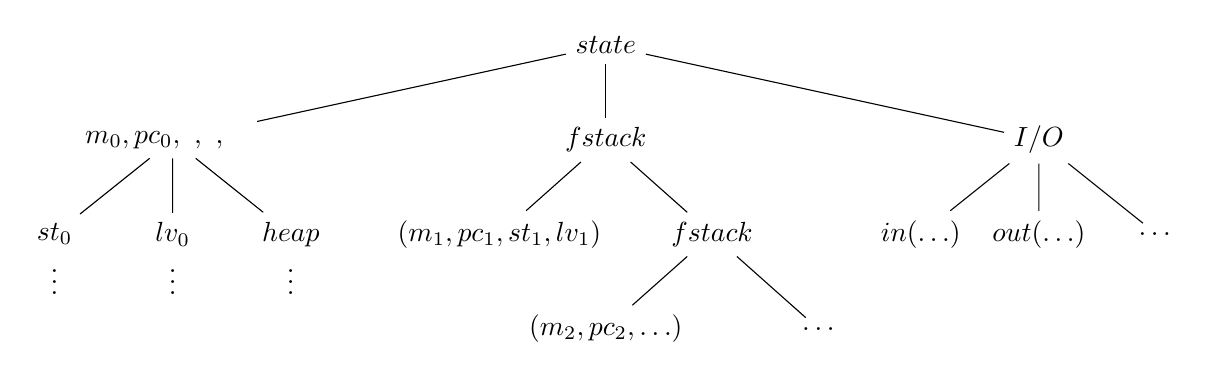
\begin{tikzpicture}[level distance=12mm, scale=1]
      \tikzstyle{level 1}=[sibling distance=55mm]
      \tikzstyle{level 2}=[sibling distance=27mm]
      \node{$state$}%[grow=right]
      child{node{$\la m_0, pc_0,\ ,\ ,\ \ra\quad$}
        child[sibling distance=15mm]{node{$st_0$} child[draw=white, level distance=5mm]{node{\vdots}}}
        child[sibling distance=15mm]{node{$lv_0$} child[draw=white, level distance=5mm]{node{\vdots}}}
        child[sibling distance=15mm]{node{$heap$} child[draw=white, level distance=5mm]{node{\vdots}}}
      }
      child{node{$fstack$}
        child{node{$(m_1, pc_1, st_1, lv_1)$}
        }
        child{node{$fstack$}
          child{node{$(m_2, pc_2, \dots )$}}
          child{node{$\dots$}}
        }
      }
      child{node{$I/O$}
        child[sibling distance=15mm]{node{$in(\dots)$}}
        child[sibling distance=15mm]{node{$out(\dots)$}}
        child[sibling distance=15mm]{node{\dots}}
      };
    \end{tikzpicture}
  }
  \caption{\footnotesize Un état de la JVM représenté comme un terme}
  \label{fig:etat-terme}
\end{figure}

L'outil \emph{Copster} produit deux types de règles de réécriture à
partir du programme qui lui est fourni en entrée. Une partie des règles est propre
au programme : ces règles permettent d'établir le séquencement des
instructions de chaque méthode. Le seconde catégorie de règles est
propre à la sémantique opérationnelle de Java et modélise les
différentes instructions du langage.
% et d'autre part un ensemble de règle modélisant le programme.
Cette seconde catégorie de règles constitue une base fixe et commune à tous
les programmes modélisés sous forme par les systèmes de réécriture générés.
La figure~\ref{fig:semantique-java} donnent deux exemples de règles
sémantiques pour des instructions du ByteCode Java.

\begin{figure}[ht!]
  \centering
  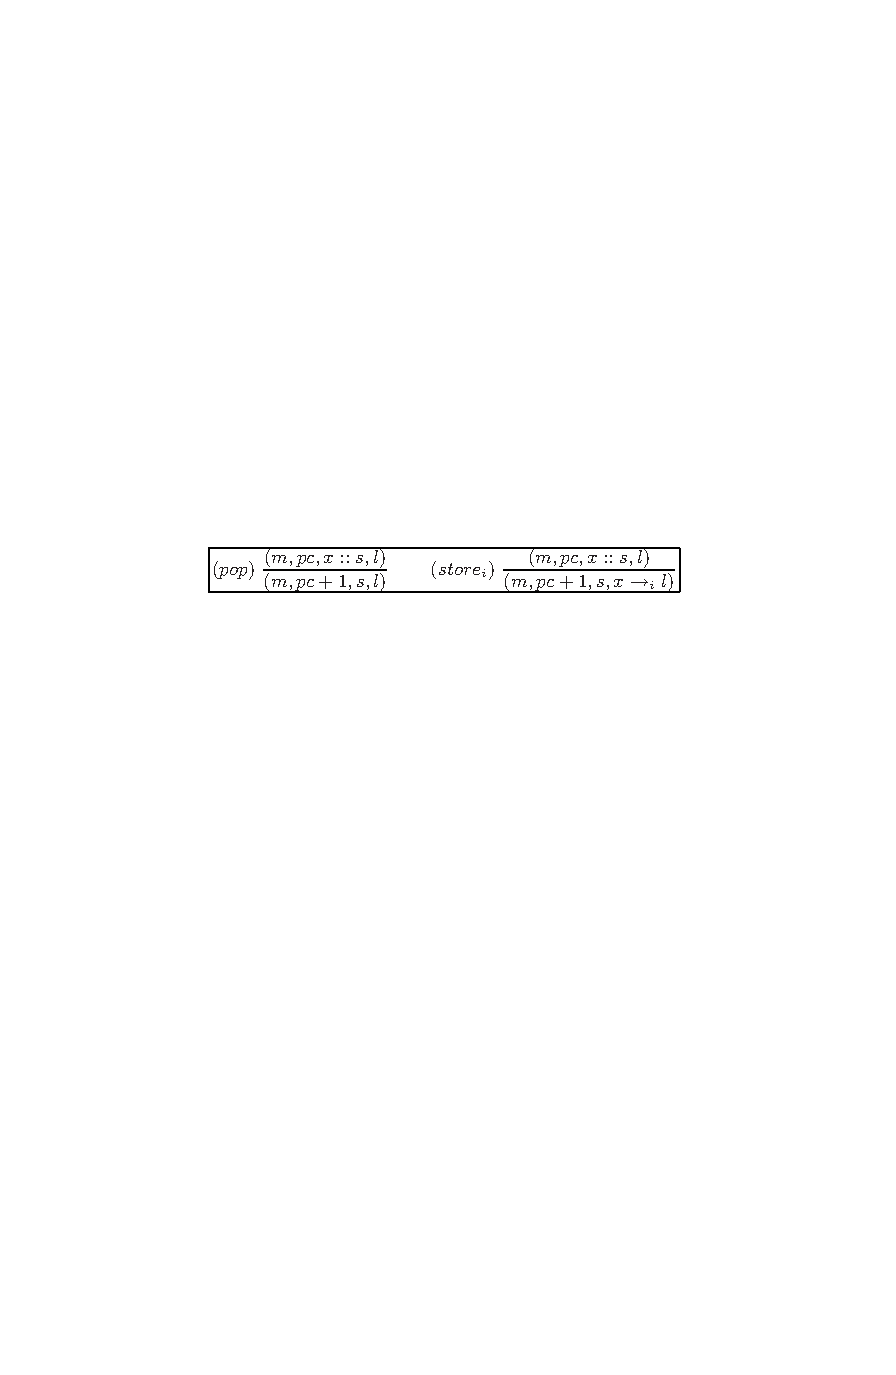
\includegraphics[scale=1.3]{jvm_1}
  \caption{\footnotesize Extrait de la sémantique opérationnelle du ByteCode Java}
  \label{fig:semantique-java}
\end{figure}

On peut noter qu'en fonction de la nature des instructions, les règles
de la sémantique n'ont d'impact que sur une partie de l'état de la
machine virtuelle. Ainsi, la majorité des instructions ($\kw{store_i}$,
$\kw{aload\_0}$, $\kw{goto}$, $\kw{if\_icmpe}$, \dots) du ByteCode,
ne portent que sur le contexte de la méthode courante et/ou sur le tas
($\kw{get\_field}$, $\kw{put\_field}$. Cependant, les instructions
dédiées aux appels et retour de méthodes ($\kw{invokeVirtual}$, $\kw{return}$, \dots)
modifient la pile d'appel en plus du contexte de la méthode courante et
concerne une plus grande partie de l'état de la machine virtuelle.

Le système de réécriture généré par \emph{Copster} pour un programme
donné assure un certain nombre de bonnes propriétés issues de la
sémantique. Principalement, le système de réécriture produit est toujours
linéaire à gauche, déterministe, et préserve la séquentialité
des instructions de telle sorte qu'il n'existe qu'une seule manière de
réécrire chaque terme atteignable.  Le comportement de chaque
instruction est simulé par un ensemble de règles équivalent à la règle
sémantique. On peut voir dans la figure~\ref{fig:semantique-trs} qu'il suffit
de trois règles pour exécuter l'instruction au point de programme $pc_1$ de la méthode
$\kw{C.m1()}$. La règle (2) est la simple traduction de la règle sémantique de $\kw{pop}$,
alors que les règles (1) et (3) sont dédiées à la méthode $\kw{C.m1}()$, et donc propres au 
programme. La règle (1) permet de lier au point de programme $pc_1$ de $\kw{C.m1}()$ l'instruction
correspondante : $\kw{pop}$. On voit que la règle (1) convertit le contexte en un contexte intermédiaire $xframe(\dots)$
sur lequel est défini la sémantique des instructions. Une fois l'exécution terminée, un nouveau 
contexte $frame(\dots)$ est produit. La règle (3) incrémente simplement l'index de l'instruction à exécuter.

\begin{figure}[ht!]
  \centering
  \[
  {%\footnotesize
    \begin{array}{|c|ll|}
      \hline
      1 & frame(name(m1, C), pc1, st, lv, h) & \lrw xframe(pop, name(m1, C), pc_1, st, lv, h)\\
      2 & xframe(pop, m, pc, stack(x, s), l, h) & \lrw frame(m, next(pc), s, l, h) \\
      3 & next(pc_1) &\lrw pc_2 \\
      \hline
    \end{array}
  }
  \]
  \caption{\footnotesize Règles pour l'instruction $\kw{pop}$ de la méthode $\kw{C.m1()}$}
  \label{fig:semantique-trs}
\end{figure}


Un point crucial pour la suite est la possibilité de déterminer une
classification des règles. En effet, la position à laquelle peut
réécrire une règle de réécriture dans un terme détermine la nature
sémantique de la règle. En se focalisant sur une position donnée du
terme, on peut alors analyser les séquences de réécriture
correspondant aux graphes d'appels des méthodes Java, les opérations
réalisées sur le tas \textit{etc}\dots\ On va donc montrer comment
exploiter cette propriété du langage pour réaliser une analyse
inter-procédurale du flot de contrôle pour des programmes Java.

\subsection{Chaîne de réécriture à la position $p$}

On considère $\R$ le système de règles de réécriture, et un ensemble d'équations $E$.
On va définir $\arw_{\R_p/E}$ une sous relation de $\rw_\RE^*$ la
relation de réécriture induite par $\RE$.  Le but de la relation
$\arw_{\R_p/E}$ est de caractériser la réécriture uniquement par les
étapes de réécriture qui ont lieu à la position $p$.

\begin{definition}
  \label{def:arw}
  Soient $s,\ t \in \TF$ deux termes tels que $s \rw_\RE^* t$.
  Soit $p \in \pos(s)$ une position de $s$. Alors on a \textbf{$s \arw_{\R_p/E} t$} si et seulement si
  il existe un terme $w$ qui satisfait les conditions suivantes:
  \begin{itemize}
  \item  $s \rw_\RE^* w$
  \item $w$ doit être obtenu par réécriture uniquement de sous-termes stricts de $s|_p$.
  \item $t=_E w[r\sigma]_p$ avec $l\rw r \in \R$ et $w|_p = l\sigma$
  \end{itemize}
\end{definition}

Dans le cas où l'ensemble des équations est vide, on note par $\arw_{\R_p}$ la relation $\arw_{\R_p/\emptyset}$.
De la même manière on utilise la notation $\arw_\RE$ pour $p = \epsilon$. Ce qui nous donne au final, la notation
$\arw_\R$ dans le cas $p = \epsilon$ et $E = \emptyset$.
On voit par l'intermédiaire de l'exemple~\ref{ex:arw}, que la relation $\arw_{\R_p}$ permet 
d'abstraire la séquence de réécriture: les différents étapes de réécriture nécessaires
pour arriver à l'étape de réécriture à la position $p$ sont simplement oubliées.
De ce fait, on ne conserve que les termes qui sont produits par la réécriture à la position $p$.
\begin{example}
  \label{ex:arw}
  On considère la séquence de réécriture suivante. A chaque étape, le
  sous-terme réécrit est souligné, et le sous-terme produit est en
  gras.
  \begin{multline*}
    f(g(\underline{a}), h(b)) \lrw_\R 
    f(\underline{g(\textbf{b})}, h(b)) \lrw_\R 
    f(\textbf{h(\underline{b})}, h(b)) \lrw_\R
    \\
    \\
    f(\textbf{a}, h(\underline{b})) \lrw_\R 
    f(a, \underline{h(\textbf{c})}) \lrw_\R 
    \underline{f(a, \textbf{a})} \lrw_\R 
    \textbf{g(f(a, a))} %\rw_\R 
    % \textbf{f(a, f(a, \underline{a})}) \rw_\R  %doit remplacer celle du dessus
    % f(a, f(a, \textbf{b}))
  \end{multline*}
  conformément à la définition~\ref{def:arw} on peut exhiber les relations suivantes:
  
  \medskip
  \begin{itemize}
  \item $f(g(a), h(b)) \arw_{\R_1} f(h(b), h(b))$
  \item $f(a, h(b)) \arw_{\R_2} f(a, a)$
  \item $f(g(a), h(b)) \arw_\R g(f(a,a))$
  \end{itemize}
\end{example}

Dans le cas où le système de réécriture modélise l'exécution d'un programme Java, la position de réécriture
permet de caractériser la nature sémantique l'étape de réécriture.
Si l'on considère $s$ un état conforme à la figure~\ref{fig:etat-terme} aux positions suivantes, on peut considérer:

\begin{itemize}
\item Le sous-terme $s|_1 = \la m_0, pc_0, \dots \ra$ est le contexte
  de la méthode en cours. La réécriture à la position $1$ correspond au début de
  l'exécution des instructions du ByteCode.

\item La réécriture aux positions $s|_{13}$ et $s|_{14}$ correspond
  aux opérations élémentaires comme la modification de la pile ou des
  variables locales\dots
  
\item Plus intéressant, le sous-terme~$s|_{15}$ correspond au tas: les
  règles de réécriture appliquées à cette position concerne la
  consultation, la création ou la modification des objets ou tableaux
  stockés en mémoire.

\item Le sous-terme $s|_\epsilon$ soit $s$ lui-même, est réécrit par les
  règles qui correspondent aux appels et retours de méthodes.
\item \dots
\end{itemize}

On considère maintenant un état de la machine virtuelle correspondant
au début de l'exécution d'une méthode $m$ donnée par le contexte $f_0 =
\la m, pc_0, \epsilon, lv_0, h_0\ra$, une certaine pile d'appels $fs$
et des entrées et sorties de la forme $I/O(\dots)$.  Cet état est la
forme $s_0 = state(f_0, fs, I/O(\dots))$. Si on déroule l'exécution de
la méthode \emph{pas à pas} de l'instruction $\kw{instr}_i$ au point de
programme $pc_i$ on obtient un nouveau contexte $f_{i+1}$ par
réécriture. L'exécution de l'instruction débute par la réécriture de
l'état $s_i$ à la position $1$, ce qui construit un état intermédiaire, sur
lequel a lieu toutes les étapes de réécriture nécessaires pour
réaliser les différentes manipulations (sur les variables, la pile, le
tas) induites par l'exécution de l'instruction $\kw{instr}_i$. Comme
indiqué ci-dessus, ces étapes de réécriture ont lieu uniquement sur
les sous-termes de $f_i$: %situés aux positions $1[1..9]^*$:

\[ state(\underline{f_i}, fs, I/O(\dots)) \lrw_\R^* state(\mathbf{f_{i+1}}, fs, I/O(\dots)) \]

Si le point de programme $p_n$ correspond à un appel de la méthode
$m'$ qui va produire un nouvel état de la forme $state(f'_0, fs',
I/O(\dots))$ où le contexte est de la forme $f'_0 = \la m', pc_0,
\epsilon, lv'_0, h_n \ra$ et la pile $fs' = fstack((m, pc_n, st_n,
lv_n), fs)$. Au final, on obtient la séquence de réécriture suivante:
\begin{multline*}
  state(\underline{f_0}, fs, I/O(\dots)) \lrw_\R^* \underline{state(\mathbf{f_n}, fs, I/O(\dots))} \\
  \lrw_\R \mathbf{state(f'_0, fstack((m, pc_n, st_n, lv_n), fs), I/O(\dots))}  
\end{multline*}

\noindent qui peut être abstraite:
\[ state(f_0, fs, I/O(\dots)) \quad \arw_\R \quad state(f'_0, fstack((m, pc_n, st_n, lv_n), fs), I/O(\dots)) \]
Puisque $f_0$ et $f'_0$ représentent respectivement les états au point d'entrée des méthodes $m$ et $m'$, la relation ci-dessus
dénote bien à l'appel de la méthode $m'$ par $m$. Ainsi, les traces d'exécutions abstraites par la relation $\arw_\R$
permettent de construire le graphe d'appels d'un programme Java.
Ce graphe inter-procédural peut-être obtenu par la complétion d'un automate d'arbres.
En fait l'automate étant souvent obtenu par une sur-approximation paramétrée par $E$ un ensemble d'équations, il caractérise 
un sous-ensemble de la relation plus générale $\arw_{\R_p/E}$. 

\section{Completion d'automates d'arbres et $\arw_{\R_p/E}$}

La relation $\arw_{\R_p/E}$ que l'on cherche à caractériser est en fait construite
et maintenue naturellement par la complétion. Elle est intrinsèquement liée à la nature
des automates d'arbres et finalement à la manière dont sont ajoutées les  $\varepsilon$-transitions 
par les étapes de complétion. En effet, chaque $\varepsilon$-transition de la forme $q' \rw q$
met en relation les représentants de $q'$ et $q$ par $\arw_{\R_\epsilon/E}$.
Ce qui nous donne la propriété suivante~:

\begin{lemma}
  \label{lem:completion_arw}
  Soit $\A = \la \F, \Q, \Q_f, \Delta \cup \Deps\ra$ un automate obtenu 
  par complétion à partir des règles $\R$ et des équations $E$.
  Alors pour toute transition $q' \lrw q \in \Deps$ de $\A$,
  et tous les représentants de $q$ et $q'$:
  \[
  \xymatrix{
    u \ar[dd]_{\A}^{\not\varepsilon} \ar@{-->} [rr]_{\R/E} && v \ar[dd]^{\A}_{\not\varepsilon}\\
    &&\\
    q && q' \ar[ll]
  }
  \]
  
  \end{lemma}

\begin{proof}
  La preuve se base sur la définition~\ref{def:re-coherence} de la $\RE$-cohérence qui est plus forte.
  Elle assure que pour tout état $q$ d'un automate produit par complétion, si $s \in \Rep (q)$ est un représentant de l'état $q$
  alors~:
  \begin{itemize}
  \item $\forall t \in \Rep(q)$, $s =_E t$
  \item $\forall t \in \Lang(\A, q)$, $s \rw_\RE^* t$.
  \end{itemize}

  On considère la transition $q \rw q' \in \Deps$. Par construction, cette $\varepsilon$-transition est ajoutée
  par la résolution de la paire critique $\la q, r\sigma\ra$ formée par l'automate avec une règle $l\rw r \in \R$.
  On rappelle que la substitution $\sigma$ associe à chaque variable $x$ du membre gauche $l$ un état $\sigma(x) \in \Q$
  telle que:
  \[
  \xymatrix{
    l\sigma \ar[dd]^{\A}_{*} \ar[rr]_{\R}  & & r\sigma\\ % \ar[dd]^{\aaexeq^{k+1}}_{\not\varepsilon}\\
    & & \\
    q & &% q' \ar[ll]^{\aaexeq^{k+1}}
  }
  \]
  Une telle paire critique a été résolue en ajoutant à l'automate les transitions $r\sigma \rwne q'$ et $q' \rw q$.
  Ensuite on considère la substitution $\sigma' : \X \rw \TF$ de la forme
  $\{ x \mapsto \sigma'(x) \sep \sigma'(x) \in \Rep(\sigma(x)) \}$. On a automatiquement $l\sigma' \rw_{\A}^* l\sigma$ :
  l'ensemble des substitutions $\sigma'$ dénotent les termes $l\sigma'$ reconnus en $q$ qui sont réécrits par la règle $l \rw r$ 
  tels que  $r\sigma'$ est un représentant de $q'$ puisque l'on a $r\sigma' \rwne_{\A} r\sigma$.

  Grâce au premier point de la définition~\ref{def:re-coherence} et la résolution de la paire critique
  on obtient le diagramme suivant:
  \[
  \xymatrix{
    u \ar[rr]_{\RE^*} \ar@/_2pc/[rrdd]^{\not\varepsilon}_{\A} & & l\sigma' \ar[dd]^{\A}_{*} \ar[rr]_{\R}  & & r\sigma' \ar[dd]^{\A}_{\not\varepsilon}\\
    & & & & \\
    & & q & & q' \ar[ll]^{\A}
  }
  \]
  où $u$ est un terme représentant quelconque de $q$. On obtient donc une chaîne de réécriture entre les termes $u$ et $r\sigma'$
  dont la dernière étape de réécriture est réalisée à la position $\epsilon$. De plus, 
  $u$ et $r\sigma'$ sont respectivement des représentants de états $q$ et $q'$.

  Pour établir la relation $u \arw_\RE r\sigma'$, il
  suffit de montrer qu'il n'y a aucune étape de réécriture située à la
  position $\epsilon$ sur $u \rw_\RE^* l\sigma'$.  Pour cela, il faut
  regarder une caractéristique de l'algorithme de filtrage: si
  $\sigma$ est une solution du problème de filtrage $l \match q$,
  alors on sait que $l\sigma \rw_\A^* q$.  Cependant, pour des raisons
  d'optimalité, la dernière transition utilisée pour réécrire
  $l\sigma$ en $q$, est une transition normalisée de $\Delta$, donc de
  la forme $f(q_1,\dots, q_n) \rw q$.  Il est suffisant de considérer
  ce cas pour que la paire critique soit aussi résolue pour tous les
  états dans lesquels $q$ peut-être réécrit: avoir $r\sigma \rw_\A^*
  q$ est suffisant pour obtenir la transition $r\sigma \rw_{\A}^* q''$
  pour toute paire critique $\la l\sigma, q'' \ra$ avec $q \rw_{\A}^*
  q''$ à partir d'une transition de la forme $l\sigma \rw^*_{\A} q
  \rw^*_\A q''$.
  
  On peut donc en déduire que tout terme $l\sigma'$ est un terme de la forme $f(t_1, \dots, t_n)$ tels que 
  pour chaque sous-terme on ait $t_i \rw_\A^* q_i$. D'après le premier point de la $\RE$-cohérence,
  on peut construire un terme $s_i$ représentant de $q_i$ tel que $s_i \rw_\RE^* t_i$. 
  Par composition, $f(s_1, \dots, s_n)$ est un représentant de l'état $q$:
  on a $ f(s_1,\dots, s_n) \rwne_\A f(q_1,\dots, q_n)$ et $f(q_1,\dots, q_n) \rw q \in \Delta$.
  On peut produire le terme $l\sigma'$ par réécriture des sous-termes stricts de $f(s_1, \dots, s_n)$.

  De plus, comme le terme $u$, le terme $f(s_1, \dots, s_n)$ est un représentant de $q$. En adéquation
  avec le second point de la $\RE$-cohérence, on peut en déduire que $u =_E f(s_1, \dots, s_n)$.
  De même $r\sigma'$ est un représentant de $q'$: donc pour tout représentant $v$ de $q'$ on a $r\sigma' =_E v$
  Finalement, cela permet de conclure la preuve puisqu'on a $u \rw_\RE^* l\sigma' \rw_\R r\sigma' =_E v$
  avec $l\sigma'$ obtenu uniquement par des étapes de réécriture sur des sous-termes stricts:

  \[
  \xymatrix{
    &&&&&\\
    u \ar@/_2pc/[rrdd]^{\not\varepsilon}_{\A} \ar[rr]_{\RE}^{*} \ar @/^1.8pc/ @{-->} [rrrrrr]^{\RE} &&
    l\sigma' \ar[dd]^{\A}_{*} \ar[rr]_{\R}&&
    r\sigma' \ar[dd]^{\A}_{\not\varepsilon} && v \ar@{=}[ll]^{E} \ar@/^2pc/[lldd]_{\not\varepsilon}^{\A}\\
    &&&&&\\
    && q && q' \ar[ll]^{\A} &
  }
  \]
  \noindent
  pour tout $u \in \Rep(q)$ et $v \in \Rep(q')$.
\end{proof}


\newcommand{\wrsav}{\wr}
\renewcommand{\wr}{\leftarrow}
  De cette propriété découle immédiatement la généralisation pour n'importe quelle position.
  En effet, on considère un terme $t \in \Lang(\A, q)$ tel que $t_p \in \Rep(q_1)$ et $t[q_1]_p \rw_\A^* q$:
  pour toute transition $q_2 \rw q_1\in \Deps$ alors pour tout $u_1 \in \Rep(q_1)$ on a $t \arw_{\R_p/E} t[u_1]_p$.
  Ainsi à partir de la chaîne de $\varepsilon$-transitions $q_1 \wr q_2 \wr q_3 \wr q_4 \wr \dots$,
  on peut déduire la séquence
  \[t \arw_{\R_p/E} t[u_1]_p \arw_{\R_p/E} t[u_2]_p \arw_{\R_p/E} t[u_3]_p \arw_{\R_p/E} t[u_4]_p \quad \dots\]
  \noindent avec $u_i \in \Rep(q_i)$.
\renewcommand{\wr}{\wrsav}


% The verification technique used in~\cite{BoichutGJL-RTA07}, called Tree Automata
% Completion~\cite{FeuilladeGVTT-JAR04}, is abble to finitely over-approximate the
% set of reachable terms, i.e. the set of all reachable states of the
% JVM. However, this technique lacks precision in the sense that it makes no
% difference between all those reachable terms. Due to the approximation
% algorithm, all reachable terms are considered as equivalent and the execution
% ordering is lost. This prevents, in particular, to prove temporal properties on such models. 
% However, using approximations make it possible to prove unreachability
% properties on infinite state systems.

% In this preliminary work, we propose to improve the Tree Automata Completion
% method so as to prove temporal properties on TRS representing a finite state
% system. The first step is to refine the algorithm so as to produce a tree
% automaton keeping an approximation of the rewriting relation between
% terms. Then, in a second step, we propose a way to check LTL-like formulas on
% this tree automaton.


\section{Extraction d'une structure de Kripke}
Soit $\aaexeq^*= \la \T(\F), \Q, \Q_F, \Delta \cup \Deps \ra$ un automate d'arbres obtenu par 
complétion pour $\R$ un système de réécriture donné, avec un ensemble d'équation $E$, à partir 
du langage initial~$I$. On suppose que $\aaexeq^*$ est $\R$-clos soit $\aaexeq^* \supseteq \R(\aaexeq^*)$.

Une structure de Kripke est un graphe orienté utilisé dans le model-checking pour représenter le comportement d'un système. 
Les noeuds représentent les états accessibles du système et les arcs représentent les transitions du système.
Une fonction d'étiquetage associe à chaque état l'ensemble des propriétés de cet état. 

\begin{definition}
Une structure de Kripke est un quadruplet de la forme $\K = (S, S_0, R, L)$ tel que
\begin{itemize}
\item $S$ est un ensemble d'états,
\item $S_0 \subseteq S$ est l'ensemble des états initiaux,
\item $R \subseteq S \times S$ est la relation de transition qui doit être totale à gauche,
\item $L$ est une fonction qui étiquette chaque état $s$ avec un ensemble de prédicats qui sont vrais 
  dans l'état $s$.
\end{itemize}
\end{definition}

On veut construire un tel modèle pour le sous-ensemble de la relation $\arw_{\R_p/E}$ contenu par l'automate $\aaexeq^*$
à partir d'un ensemble de termes $t_0 \in \Lang(\aaexeq^*)$. Cependant à cause du lemme~\ref{lem:completion_arw}, les sous-termes
initiaux $t_0|_p$  concernés par $\arw_{\R_p/E}$ doivent être des représentants de l'état qui les accepte :
\begin{equation*}
  \label{eq:1}
  t_0 \rwne_{\aaexeq^*} t_0[q]_p \rw_{\aaexeq^*}^* q_f,\quad \textrm{ avec } q_f \in \Q_f
\end{equation*}

On peut alors ramener le problème d'analyse de $\arw_{\R_p/E}$ à l'analyse de $\arw_{\R_p/E}$ pour les sous-termes $t_0|_p$.
Ces sous-termes sont des représentants pour l'état $q$, et l'acceptation de $t_0|_p$ par l'état $q$ est une étape dans la
reconnaissance de $t_0$ par l'automate. On note $Q_0$ l'ensemble de ces états $q$.

Pour construire le modèle de Kripke, on prend les états de l'automate comme états de la structure de Kripke, 
la fonction de transition $R$ est définie au moyen des $\varepsilon$-transitions.
Enfin l'ensemble des prédicats attachés à  chaque état est défini par l'ensemble des représentants associés à l'état. 
On définit alors la fonction de \textit{labelling} $L$ simplement par une fonction qui associe un automate d'arbres à chaque état.

\begin{definition}
  On définit la fonction de labelling $L : q \mapsto \la \F, \Q, \{q\}, \Delta\ra$ comme la fonction
  qui associe à un état $q$, l'automate $L(q)$ issu de l'automate $\aaexeq^*$ privé des $\varepsilon$-transitions
  et pour lequel $q$ est l'unique état final.
  Par construction, on peut montrer que les termes reconnus par l'automate $L(p)$ sont exactement les représentants
  de l'état $q$ dans l'automate complet $\aaexeq^*$.
  \[\forall t \in \Lang(L(q)), \quad t \rwne_{\aaexeq^*} q\]
\end{definition}

Ce qui permet alors de construire la structure de Kripke correspondant à la relation $\arw_{\R_p/E}$ pour l'ensemble des termes $t_0$.

\begin{definition}%[Construction of a Kripke Structure]
  On construit le quadruplet $(S, S_0, R, L)$ à partir de l'automate $\aaexeq^*$.
  Chaque composante du quadruplet se définit par:
  \begin{itemize}
  \item $S = \Q$, 
  \item $S_0 = Q_0$,
  \item $R(q, q')$ si $q' \rw q \in \Deps$
  \item la fonction de labelling $L$ telle que définie ci-dessus.
  \end{itemize}
\end{definition}

Cependant, une structure de Kripke doit être constituée d'une relation $R$ qui soit totale à gauche.
Ainsi pour n'importe quel état $q$ qui n'a pas de successeur par $R$, on le fait boucler sur lui-même
de façon à avoir $R(q, q)$. Cette transformation relativement classique provient du fait que
la logique temporelle CTL$^*$ utilisée pour formaliser les propriétés reposent sur des modèles dont les traces
d'exécution sont infinies.

Dans notre analyse inter-procédurale, ce sont les étapes de réécriture au sommet des termes qui caractérisent
les appels et retours de méthodes dans les programmes Java. En supposant que l'ensemble des états finals de $\aaexeq^*$ est $\Q_f$,
on veut donc obtenir un modèle pour la relation de transition induite par la relation $\arw_{\R/E}$, pour les termes $t_0 \in I$ l'ensemble initial. Ce qui implique
que l'ensemble des états initiaux $S_0$ correspond simplement à $\Q_f$, l'ensemble des états finals de 
l'automate. En effet, tout terme initial de $I$ est systématiquement un représentant d'un état final par construction.

% Une structure de Kripke est paramétrée par l'ensemble $S_0$.
% It defines which connected component of $R$ we are interested to analyze. For instance, to analyze 
% the abstract rewriting at the top position of terms in $\Lang{}(\aaex^*)$, we define
% set $S_0 = \Q_F$ (the set of final states of $\aaex^*$), since all canonical
% terms of final states are initial terms. 
% For all abstract rewriting at a deeper position $p$, we need to define 
% a set $Sub$ of initial subterms considered as the beginning of the rewriting
% at the position $p$. Then the set $S_0$ will be defined as 
% $S_0 = \{q \sep \exists t \in Sub,\; t \rwne_{\aaex^*} q\}$.
 
La structure de Kripke obtenue modélise la relation de réécriture $\arw_\RE^*$ 
à la position $p$ à partir des sous-termes $t_0|_p$.

\begin{theorem}
  Soit $\K=(S, S_0, R, L)$ la structure de Kripke extraite à partir de l'automate $\aaexeq^*$.
  Pour tous les états $s$, $s'$ tels que $R(s, s')$ soit vraie, alors pour tous les termes
  $u \in \Lang(L(s))$ et $v \in \Lang(L(s'))$ on a  $u \arw_{\RE} v$. De plus, pour tout terme $u,\ v \in \Lang(L(s))$
  de tout état $s$, on a $u =_E v$.
\end{theorem}

\begin{proof}
  Ce théorème est la conséquence immédiate du lemme~\ref{lem:completion_arw} 
  appliqué à l'automate $\aaexeq^*$ et de la définition de la relation de transition $R$.
\end{proof}



\begin{example}
  \label{the_example}
  Pour illustrer ce résultat, on propose de considérer l'automate d'arbres suivant obtenu par complétion
  à partir du système de réécriture $\R$ défini par $\{ a \rw b,\; b\rw c \} \cup \{f(c) \rw g(a),\; g(c) \rw h(a),\; h(c) \rw f(a)\}$.
  On part de l'ensemble initial $I=\{f(a)\}$.
  Sans approximation, \textit{i.e.} $E = \emptyset$, on obtient l'automate point fixe suivant~:
  {\small
    \[\aaex^*= \left\la
      \Qf = \{q_f\},\quad
      \Delta = \left\{
        \begin{array}{rcl}
          a & \rw & q_a \\
          b & \rw & q_b \\
          c & \rw & q_c \\
          f(q_a) & \rw & q_f \\
          g(q_a) & \rw & q_g \\
          h(q_a) & \rw & q_h \\
        \end{array}
      \right\}\:
      \Deps= \left\{
        \begin{array}{rcl}
          q_b & \rw & q_a \\
          q_c & \rw & q_b \\
          q_g & \rw & q_f \\
          % q_f & \rw & q_g \\
          q_h & \rw & q_g \\
          q_f & \rw & q_h \\
        \end{array}\right\}
      \:
    \right\ra
    \]
  }
  
  \noindent Si on regarde la transition $q_h \rw q_g$, et les termes $h(a)$ et $g(a)$ représentants de $q_h$ et $q_g$ respectivement, 
  on en déduit $g(a) \arw_\R h(a)$. Ce qui correspond bien à
  $g(\underline{a}) \rw_\R g(\underline{\textbf{b}}) \rw_\R \underline{g(\textbf{c})} \rw_\R \textbf{h(a)}$.
%   Dans l'exemple~\ref{the_example}, si on veut vérifier une propriété sur $\arw_\R$
%   on a besoin de seulement considérer sous-ensemble de transitions de $\Deps$ qui correspondent 
%   à l'abstraction de la relation de réécriture $\arw_\R$.
%%%%%   The subsets are quite simple 
  Les figures~\ref{fig2}~et~\ref{fig3} montrent l'extraction de la structure de Kripke à partir de l'automate
  pour les relation $\arw_{\R_1}$ et$\arw_{\R_\epsilon}$ respectivement.
  % Note that in figure~\ref{fig2}, a loop is needed on state $c$ to have a total relation
  % for $\K_1$.
  
  \begin{figure}[!ht]
    \begin{minipage}{0.5\linewidth}
      \centering
      \begin{tikzpicture}[thick, initial text=]
        \tikzstyle{every node}=[font=\tiny]
        \tikzstyle{every state}=[minimum size=.8cm]
        \tikzstyle{accepting}=[accepting by double]
        \node [initial,state] (a) at (0, 0) {$q_a$}; 
        \node [state] (b) at (2, 0) {$q_b$};
        \node [state] (c) at (4, 0) {$q_c$};
        \node [] (f) at (0, 1.8) {};
        \draw[->] (a) edge (b) (b) edge (c) (c) [loop right] edge (c);
      \end{tikzpicture}
      % 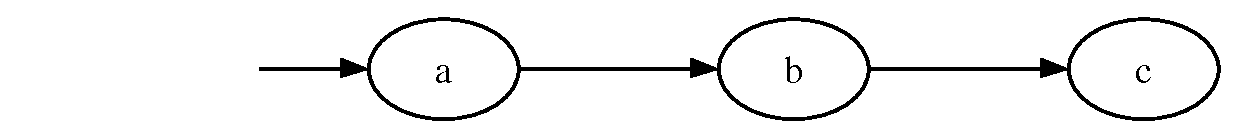
\includegraphics[scale=0.4]{R1}
      \caption{\label{fig2}\footnotesize $\K_1$ modélise $\arw_{\R_1}$}
    \end{minipage}
    \begin{minipage}{0.5\linewidth}
      \begin{center}
        \begin{tikzpicture}[thick, initial text=]
          \tikzstyle{every node}=[font=\tiny]
          \tikzstyle{every state}=[minimum size=.1cm]
          \tikzstyle{accepting}=[accepting by double]
          \node [initial,state] (a) at (0, 0) {$q_f$}; %{$f(a)$}; 
          \node [state] (b) at (2, 0) {$q_g$}; %{$g(a)$};
          \node [state] (c) at (1, 1.5) {$q_h$}; %{$h(a)$};
          \draw[->] (a) edge (b) (b) edge (c) (c) edge (a);
        \end{tikzpicture}
        % 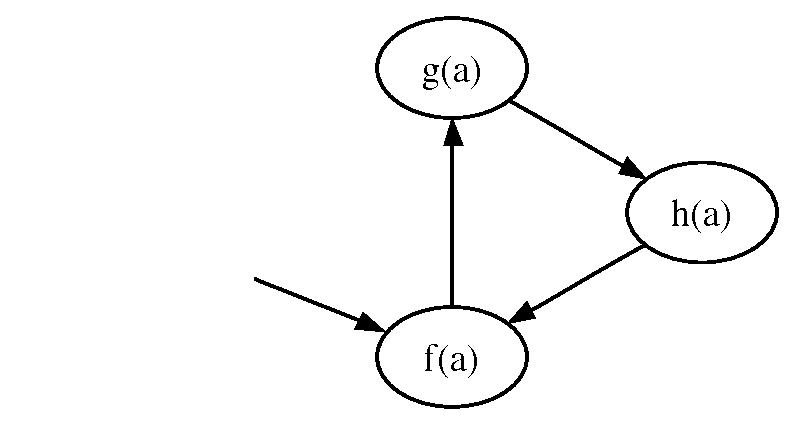
\includegraphics[scale=0.4]{R2}
        \caption{\label{fig3}\footnotesize $\K_\epsilon$ modélise $\arw_{\R_\epsilon}$}
      \end{center}
    \end{minipage}
  \end{figure}
\end{example}


% \comments{REFAIRE LES SCHEMAS : REMPLACER LES TERMES PAR DES ETATS CORRESPONDANTS
% OU ETATS (TERMES)? Moi je laisserais les termes sur cet exemple car ca permet de
% comprendre mieux ou on va. Quite a mettre les etats dans la suite de l'exemple
% et expliquer qu'ils reconnaissent ces termes.}

% The set $S_0$ of initial states depends of the abstract rewriting relation selected.
% For example, if we want to analyze $\arw_{\R_2}$ (or $\arw_{\R_1}$), we define $S_0=\{q_f\}$ (resp. 
% $S_0 = \{q_a\}$).

\section{Une logique temporelle portant des automates d'arbres}

A partir du moment où l'on obtenu un modèle de Kripke $\K = (S, S_0,
R, L)$, on a accès à l'ensemble des techniques exploitant ce type de
modèle~\cite{MC-Book}. la logique temporelle CTL$^*$ est une logique permettant
de raisonner sur les structures de Kripke, elle constitue donc la base des techniques
du model-checking. Cette logique est basée sur le dépliage des traces
d'exécution possibles à partir d'un état initial du modèle. Une trace
d'exécution est caractérisée par une séquence infinie d'états de la
forme $\pi = s_0, s_1, s_2, \dots$ telle que $(s_i, s_{i+1}) \in
R$. On utilise les notations $\pi(i)$ et $\pi^i$ pour dénoter respectivement
le $i^\text{ème}$ état $s_i$ de $\pi$, et le suffixe de $\pi$ commençant à l'état $s_i$.
Dans la suite, on va s'intéresser à la logique temporelle linéaire LTL, sous-ensemble de CTL$^*$,
pour illustrer l'adaptation des techniques de vérifications sur les modèles extraits à partir 
des automates complétés.


\subsection{La logique LTL, et les automates d'arbres}

Une des particularité de cette approche est l'étiquetage des états du modèle par des automates d'arbres.
Initialement, la logique temporelle est définie sur les différents opérateurs logiques et temporels
($\land$, $\lor$, $\neg$, $\nxt$, $\fut$, $\gbl$, $\unt$, $\rel$) à partir de prédicats qui constituent 
les formules atomiques. Si la sémantique des différents opérateurs est préservée, on modifie celles des
formules atomiques représentées les prédicats étant alors représenté par des automates d'arbres.
On propose de définir la Regular Linear Temporal Logic (R-LTL). La R-LTL est la logique LTL où les prédicats sont définis par des
automates d'arbres. Le langage d'un tel automate d'arbres caractérise l'ensemble des termes qui sont admissibles pour le prédicat.

Ainsi un état $q$ d'une structure de Kripke $\K$ valide le prédicat $P$ caractérisé
par l'automate d'arbres  $\A_p$ si et seulement si un terme $t$ reconnu par l'automate
$L(q)$ satisfait le prédicat $P$. Cela implique que le terme $t$ soit lui aussi reconnu
par l'automate $\A_P$. Ce qui nous donne la nouvelle règle sémantique:
\[\K,\ q \models P\quad \equ\quad \Lang{}(L(q)) \cap \Lang{}(\A_P) \neq \emptyset\]

L'intuition est que le langage de l'automate $\A_p$ décrit une propriété par un ensemble de termes possibles.
On peut alors reformuler la satisfiabilité du prédicat $P$ pour $t$ par une disjonction de la forme 
$\bigvee_{u \in \Lang(A_p)} t = u$.
Cela représente un avantage notable pour exprimer des motifs réguliers sur les termes. En effet, il est facile 
de construire un automate qui décrit une propriété par tous les termes de la forme $f(a, f(x, y))$.
Quant à l'automate $L(q)$, il fournit l'ensemble des termes qui sont accessibles par $\arw_\RE$.
De ce fait, il est alors raisonnable de considérer que l'état $q$ satisfait le prédicat $P$ si l'un des termes reconnus par $L(q)$ est aussi
dans le langage de $A_p$, ce qui est équivalent à $\Lang{}(L(q)) \cap \Lang{}(\A_P) \neq \emptyset$.
\begin{figure}[ht!]
  \centering
  \[\begin{array}{|lcl|}
    \hline
    \K, s \models \neg f & \equ &  \K, s \not\models f\\
    \K, s \models f_1 \lor f_2 & \equ & \K, s \models f_1 \textrm{ ou } \K, s \models f_2\\
    \K, s \models f_1 \land f_2 & \equ & \K, s \models f_1 \textrm{ et } \K, s \models f_2\\
    &\dots&\\
    \hline
    \K, \pi \models f & \equ & \K, \pi(0) \models f\\
    \K, \pi \models \nxt g & \equ & \K, \pi^1 \models g\\
    \K, \pi \models \fut g & \equ & \exists k \ge 0,\ \K \pi^k \models g \\
    \K, \pi \models \gbl g & \equ & \forall i \ge 0,\ \K \pi^i \models g \\
    &\dots&\\
    \hline
  \end{array}\]
  \caption{Principaux connecteurs logiques de LTL}
  \label{fig:operateursLTL}
\end{figure}
La figure~\ref{fig:operateursLTL} présente un sous-ensemble des
connecteurs logiques de LTL. On peut y distinguer deux types de
formules, celles comme $f$, $f_1$, $f_2$ qui portent sur les états
et les formules comme $g$ qui portent sur une séquence d'états.  Dans le chapitre~3
de~\cite{MC-Book}, on trouve le détail de la sémantique de tous les
opérateurs, ainsi que les règles de construction des formules en LTL.


Les transitions de la structure $K$ dénotent les étapes de réécriture abstraite $\arw_{\RE}$
plutôt que sur la relation de réécriture $\rw_\RE$. Comme la sémantique des opérateurs est définie
sur la relation de transitions de $K$, les propriétés que l'on peut exprimer et vérifier portent bien
sur la relation $\arw_\RE$.
% Note that temporal properties do not range over the 
% rewriting relation $\rw_\R$ but over its abstraction $\arw_\R$.
% It means that the semantics of the temporal operators has to be interpreted
% w.r.t. this specific relation. 

Par exemple, la formule\footnote{\footnotesize Par soucis de simplicité dans les 
  petits exemples, plutôt que de représenter chaque prédicat par un automate, on représente directement 
  l'ensemble des termes que devrait accepter l'automate caractérisant le prédicat.}
  $\gbl(\{f(a)\} \imp \nxt \{g(a)\})$ sur $\K_\epsilon$ (\textit{c.f.} figure~\ref{fig3}) : la formule
doit être interprétée comme pour tout $q$ $q'$, si $\K_\epsilon,\ q \models \{f(a)\}$ et $R(q, q')$ alors
on a  $\K_\epsilon,\ q' \models \{g(a)\}$. D'un point de vue de la réécriture par~$\R$ (exemple~\ref{the_example}), le seul terme
$u$ tel que $f(a) \arw_{\R_\epsilon} u$ est $u = g(a)$.


\subsection{Les automates de Büchi}


Les propriétés en logique LTL peuvent être vérifiées au moyen de la théorie des automates de Büchi.
Les automates de Büchi~\cite{Buchi} sont des automates finis qui reconnaissent des mots de taille infinie. 
Les mots infinis vont permettre de représenter les comportements du modèle dont les traces d'exécution
sont infinies. La structure des automates de Büchi est équivalente à celle des automates de mots finis.

\begin{definition}
  Un automate de Büchi se définit comme un quintuplet de la forme $\B = \la \Sigma, \Q, \Delta, \Q_0, \F\ra$
  avec
  \begin{itemize}
  \item $\Sigma$, un alphabet
  \item $\Q$, un ensemble d'états 
  \item $\Delta \subseteq \Q \times \Sigma \times \Q$, la relation de transition
  \item $\Q_0 \subseteq \Q$ et $\F \subseteq \Q$, les états initiaux et acceptants respectivement.
  \end{itemize}
\end{definition}
Un mot infini $w \in \Sigma^\omega$ est un mot qui contient un nombre
infini de répétitions\footnote{\footnotesize La répétition infinie est
  caractérisée par l'exposant $\omega$}. Il est accepté par un
automate de Büchi si et seulement si il existe une exécution infinie à
partir d'un état initial et qui passe infiniment souvent par un état
acceptant.

\begin{example}
  Exemple d'automate de Büchi:\\

%  \begin{tabular}{cp{10cm}}
 %   \begin{minipage}{5cm}
  \begin{center}
    \begin{tikzpicture}[scale=.8,thick,initial text=]
      \tikzstyle{every node}=[font=\tiny]
      \tikzstyle{every state}=[minimum size=.1cm]
      \tikzstyle{accepting}=[accepting by double]
      % 
      \node [initial,state] (q1) at (0, 0) {$1$}; 
      \node [accepting, state] (q2) at (4, 0) {$2$};
      % 
      \path[->]
      (q2)  edge [loop right] node {$b$} (q2) 
      edge [bend left] node [above] {$c$} (q1)
      (q1)  edge [bend left] node [above] {$a$} (q2);
    \end{tikzpicture}
  \end{center}
    % \end{minipage}
    % \hspace{1cm}
    % &
  L'automate ci-contre reconnaît le langage $\omega$-régulier $a(b^*ca)^\omega$,
  soit des mots infinis de la forme $acabbbbcabbca\dots$ par exemple.
  % \end{tabular}
\end{example}



Pour vérifier que le modèle $\K$ satisfait la propriété $P$ exprimée en R-LTL, 
il faut construire deux automates de Büchi $\B_\K$ et $\B_P$ qui acceptent respectivement
tous les comportements du modèle, et tous les comportements spécifiés par $P$.
La procédure de vérification revient alors à s'assurer que tous les comportements du modèle
$K$ sont couverts par la spécification $P$, ce qui se traduit par $\Lang(\B_\K) \subseteq \Lang(\B_P)$.
La manière standard de vérifier l'inclusion revient à vérifier qu'aucun comportement de
$\K$ ne viole $P$:
\[ \Lang(\B_\K) \cap \overline{\Lang(\B_P)} = \emptyset \]

Bien sûr, la vacuité du langage est décidable pour les automates de
Büchi, et ils sont clos par intersection et complémentation~\cite{Buchi}.

Il suffit de construire l'automate $\B_\K$ et l'automate $\overline{\B_P}$ qui reconnaît le langage $\overline{\Lang(\B_P)}$.
L'alphabet $\Sigma$ est constitué par les langages réguliers de termes de $\TF$ dénotés par les 
automates d'arbres.

\begin{definition}
  A partir du modèle $\K = (S, S_0, R, L)$, on définit l'automate de Büchi
  qui reconnaît tous les comportements de $\K$ comme $\B_\K =\la \Sigma, S \cup \{\iota\}, \Delta, \{\iota\}, S \cup \{\iota\}\ra$
  tel que $\Sigma = 2^\TF$, l'état initial est $\iota \not\in S$, et on a les transitions $(s, L(s'), s') \in \Delta$ si et seulement si $(s, s') \in R$.
  De plus, on ajoute à $\Delta$ les transitions $(\iota, L(s), s)$ pour tout état $s \in S_0$.
\end{definition}
Par construction tous les états de $\B_\K$ sont finals, pour permettre à tout chemin infini
de la structure de Kripke d'être un mot reconnu par $\B_\K$.
Si $\pi=s_0s_1s_2s_3\dots$ est une séquence valide d'états dans la structure de Kripke,
alors le mot $\pi' = L(s_0)L(s_1)L(s_2)\dots$ est reconnu par $\B_\K$.
Ce mot $\pi'$ dénote l'ensemble de séquence de réécriture de la forme
$t_0 \arw_\RE t_1 \arw_\RE t_2 \arw_\RE \dots$ tels que $t_i \in \Lang(L(s_i))$.

\begin{example}
  La figure~\ref{fig5} définit l'automate de Büchi qui pour la figure de Kripke $\K_\epsilon$:
  \begin{figure}[ht!]
    \begin{minipage}{0.5\linewidth}
      \begin{center}
        \begin{tikzpicture}[thick, initial text=]
          \tikzstyle{every node}=[font=\tiny]
          \tikzstyle{every state}=[minimum size=.1cm]
          \tikzstyle{accepting}=[accepting by double]
          \node [initial,state] (a) at (0, 0) {$q_f$}; %{$f(a)$}; 
          \node [state] (b) at (2, 0) {$q_g$}; %{$g(a)$};
          \node [state] (c) at (1, 1.5) {$q_h$}; %{$h(a)$};
          \draw[->] (a) edge (b) (b) edge (c) (c) edge (a);
        \end{tikzpicture}
        % 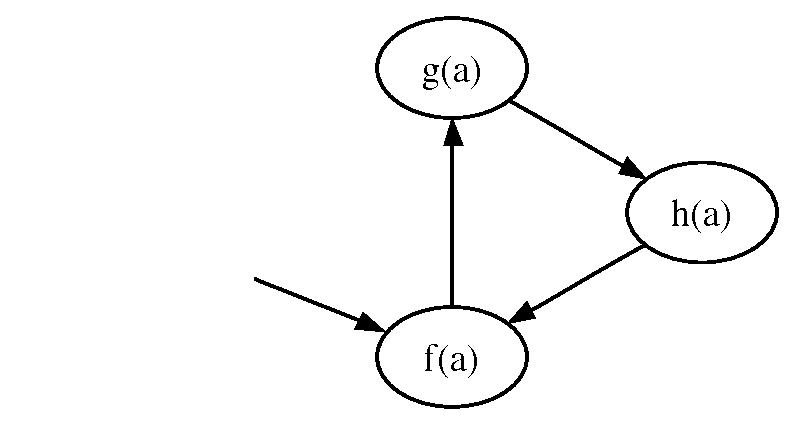
\includegraphics[scale=0.4]{R2}
      \end{center}
    \end{minipage}
    \begin{minipage}{0.5\linewidth}
      \begin{center}
        \begin{tikzpicture}[scale=.8,thick,initial text=]
          \tikzstyle{every node}=[node distance=40,font=\tiny]
          \tikzstyle{accepting}=[accepting by double]
          \tikzstyle{every state}=[accepting, minimum size=.1cm]
          % 
          \node [initial,state] (q4)            {$4$}; 
          \node [state] (q5) [right of=q4]      {$5$};
          \node [state] (q6) [below of=q5]      {$6$};
          \node [state] (q7) [right of=q6]      {$7$};
          % 
          \path[->]
          (q4)  edge []                         node [above]    {$L(q_f)$} (q5) 
          (q5)  edge []                         node [left]     {$L(q_g)$} (q6)
          (q6)  edge []                         node [below]    {$L(q_h)$} (q7)
          (q7)  edge [bend angle=40,bend right] node [right]    {$L(q_f)$} (q5);
        \end{tikzpicture}
      \end{center}
    \end{minipage}
    \caption{\footnotesize Construction l'automate $\B_{\K_\epsilon}$ pour le modèle $\K_\epsilon$}
    \label{fig5}
  \end{figure}
\end{example}

On ne s'étendra pas ici sur les techniques permettant de construire l'automate de Büchi $\overline{\B_P}$ dénotant
la négation de la formule LTL $P$, mais il est possible de trouver les détails de l'algorithme pour construire ce type
d'automate dans~\cite{DBLP:conf/pstv/GerthPVW95}.
\begin{example}
  Soit la formule $P = \gbl(\{f(a)\} \imp \nxt \{g(a)\})$.
  L'automate $\overline{\B_P}$ (fig.~\ref{fig4}) reconnaît la négation de la formule $P$
  exprimée par $\fut(\{f(a)\} \land \nxt \neg\{g(a)\})$ et $\B_\K$ (fig.~\ref{fig5}) 
  reconnaît l'ensemble des comportements de la  structure de Kripke
  $\K_\epsilon$~(fig.~\ref{fig5}). La notation $\A_\alpha$ dénote l'automate d'arbres tel que son langage est décrit par $\alpha$
  ($\A_{\neg g(a)}$ reconnaît le complément du langage $\Lang{}(\A_{g(a)})$ et $\A_*$ reconnaît tout terme de $\TF$).
  \begin{figure}[ht!]
    \centering
    % \bar{\B_L}
    \begin{tikzpicture}[scale=.8,thick,initial text=]
      \tikzstyle{every node}=[font=\tiny]
      \tikzstyle{every state}=[minimum size=.1cm]
      \tikzstyle{accepting}=[accepting by double]
      % 
      \node [initial,state] (q1) at (0, 0) {$1$}; 
      \node [state] (q2) at (2, 0) {$2$};
      \node [accepting, state] (q3) at (4, 0) {$3$};
      % 
      \path[->]
      (q1)  edge [loop above] node {$\A_*$} (q1) 
      edge node [above] {$\A_{f(a)}$} (q2)
      (q2)  edge node [above] {$\overline{\A_{g(a)}}$} (q3)
      (q3)  edge [loop above] node {$\A_*$} (q3);
    \end{tikzpicture}
    \caption{\footnotesize L'automate $\overline{\B_P}$}
    \label{fig4}  
  \end{figure}
\end{example}

% For example, the formula $\gbl(\{f(a)\} \imp \nxt \{g(a)\})$
% on $\K_2$ (for more clarity, we note predicates as sets of terms): the formula 
% has to be interpreted as : for all $q$ $q'$, if $\K_2,\ q \models \{f(a)\}$ and $R(q, q')$ then
% we have  $\K_2,\ q' \models \{g(a)\}$. In the rewriting interpretation the only term $u$ such
% that $f(a) \arw_{\R_2} u$ is $u = g(a)$.

% On utilise les automates de Büchi pour réaliser la vérification de la propriété.
% La théorie des automates de Büchi et cette technique sont détaillées dans le chapitre~9
% de~\cite{MC-Book}. Comme les formules LTL, il est possible de traduire les formules R-LTL
% ainsi que la structure de Kripke en automates de Büchi.
% On construit alors deux automates de Büchi: $\B_\K$ obtainu obtenu à partir de la structure
% de Kripke et $\B_L$ défini par la formule R-LTL qui décrit la propriété.
% Comme l'ensemble des exécutions possible de la structure de Kripke est le langage accepté
% par l'automate $\B_\K$, la structure de Kripke satisfait la formule R-LTL si 
% toutes ses traces d'exécution sont reconnues par l'automate $\B_L$.
% Cela signifie qu'il faut vérifier $\Lang(\B_\K) \subseteq \Lang(\B_L)$. 
% Pour cela, l'approche standard consiste à construire l'automate $\overline{\B_L}$ 
% qui reconnaît l'ensemble des traces qui ne satisfont pas la formule $L$:
% ce qui corespond au langage $\overline{\Lang(\B_L)}$. Ensuite il suffit de 
% vérifier la vacuité de l'automate $\B_\cap$ qui reconnaît l'intersection des 
% langages $\Lang(\B_K)$ et $\overline{\Lang(\B_L)}$. Si cette intersection
% est vide, the term rewriting system satisfait la propriété.
% C'est l'application de la technique de model-checking standard.

% $\B_\M$ et $\B_\K$ sont classiquement définis comme des quintuplets: alphabet, états,
% états initiaux, états finaux et relation de transition.
% Généralement, l'alphabet d'un automate de  Büchi est un ensemble de prédicats.
% Puisqu'on utilise ici des automates d'arbres pour définir les prédicats, l'alphabet de
% $\B_\K$ et $\B_L$ est $\Sigma$ l'ensemble des automates d'arbres que l'on peut définir sur $\TF$. 
%  Les algorithmes
% utilisés pour construire $\B_\M$ et $\B_\K$ peuvent être trouvés dans~\cite{MC-Book}.


L'automate intersection $\B_\cap$ est obtenu en calculant le produit de automates $\B_\K$ et $\overline{\B_P}$.
Comme tous les états sont finals dans l'automate $\B_\K$, il est possible d'employer une version plus
simple du produit général d'automates de Büchi pour ce cas particulier~\cite{MC-Book}. On présente une version
adaptée de cet algorithme pour les automates de Büchi dont les transitions sont étiquetées par des automates d'arbres.

\begin{definition}[$\B_\K \times \overline{\B_P}$]
  Le produit de $\B_\K = \la \Sigma,\; \Q,\; Q_0,\; \Q,\ \Delta\ra$ par 
  $\overline{\B_P} = \la\Sigma,\; \Q',\;\Q'_0,\; \F',\ \Delta'\ra$ est défini
  \[\la \Sigma,\; \Q \times \Q',\; \Q_0 \times \Q'_0,\; \Q \times F',\; \Delta_\times\ra \]
  où $\Delta_\times$ est un ensemble de transitions $(q_\K, q_P) \xrw{(\A_\K\cap\A_P)} (q'_\K, q'_P)$ tel que $q_\K
  \xrw{\A_\K} q'_\K$ est une transition
  de $\B_\K$ et $q_P \xrw{\A_P} q'_P$ est une transition de $\overline{\B_P}$. De plus, la transition 
  est seulement valide si l'intersection entre les langages de $\A_\K$ et $\A_P$ est non vide.
  %comme attendu par la satisfiabilité d'une formule atomique en R-LTL.
  % as expected by the interpretation of the R-LTL atomic formula.
\end{definition}
L'intersection d'automates d'arbres calculée sur chaque transition de
l'automate intersection se justifie simplement.  Une transition de la forme
$s, A, s'$ pourrait être vue comme un ensemble de transitions de la
forme $s, t, s'$ où $t \in \Lang(A)$. Ainsi l'intersection placée sur
les transitions du produit $\B_\K \times \overline{\B_P}$ correspond
simplement à l'ensemble des transitions $((s_1, s_2), t, (s_1',s_2'))$
tel que $t \in \Lang(\B_\K)$ et $t \in \Lang(\B_P)$.

Enfin, la vacuité du langage $\Lang{}(\B_\cap)$ peut être vérifiée en utilisant l'algorithme
basé sur la recherche en profondeur qui assure que toute composante fortement connexe accessible à partir d'un état initial
ne contient pas d'états acceptants.


\begin{example}

  Pour illustrer l'approche, on propose de vérifier pour la formule $P
  = \gbl(\{f(a)\} \imp \nxt \{g(a)\})$ de l'exemple~\ref{the_example}.
  La figure~\ref{fig6} montre le résultat de l'intersection $\B_\cap$
  entre $\B_\K$ et $\overline{\B_P}$. Seul les états atteignables
  et les transitions valides (étiquetées par une intersection
  non vide d'automates d'arbres) sont montrées.  Comme aucun état
  atteignable de $\B_\cap$ n'est final, sont langage est vide. Cela
  signifie que toutes les traces d'exécution de $\K_\epsilon$
  satisfont $P$: en effet, le seul successeur de $f(a)$ pour
  $\arw_{\R_\epsilon}$ est $g(a)$.


\begin{figure}[ht!]
    % \bar{\B_\K}
  %\begin{minipage}{0.5\linewidth}
    \centering
    % B_\cap
    \vspace{10mm}
    \begin{tikzpicture}[scale=.8,thick,initial text=,bend angle=40]
      \tikzstyle{every node}=[node distance=50,font=\tiny]
      \tikzstyle{accepting}=[accepting by double]
      \tikzstyle{every state}=[minimum size=.1cm]
      % 
      \node [initial,state] (q14)            {$1,4$}; 
      \node [state] (q15) [right of=q14, node distance=60]     {$1,5$};
      \node [state] (q16) [below of=q15]     {$1,6$};
      \node [state] (q17) [right of=q16, node distance=60]     {$1,7$};
      \node [state] (q25) [below of=q14]     {$2,5$};
      % 
      \path[->]
      (q14) edge []                 node [above]           {$\A_* \cap L(q_f)$}       (q15)
            edge []                 node [left]            {$\A_{f(a)}\cap L(q_f)$}    (q25)
      (q15) edge []                 node [left]            {$\A_* \cap L(q_g)$}       (q16)
      (q16) edge []                 node [above]           {$\A_* \cap L(q_h)$}       (q17)
      (q17) edge [bend right]       node [right]           {$\A_* \cap L(q_f)$}       (q15)
            edge [bend left]        node [below]           {$\A_{f(a)} \cap L(q_g)$}   (q25);
    \end{tikzpicture}
    \caption{\footnotesize L'automate $\B_\cap$}
    \label{fig6}
%  \end{minipage}
\end{figure}
\end{example}




\section{Conclusion, discussion}

Dans ce chapitre, on a montré comment
% améliorer la complétion d'automates d'arbres pour
exploiter le mécanisme de relation d'ordre et préserver la relation d'ordre
entre les termes accessibles, grâce aux transitions $\varepsilon$-transitions.
On a également montré comment utiliser de la relation induite par ces transitions pour prouver des 
formules en logique temporelle linéaire sur le système de réécriture. Le chapitre traite de l'analyse 
dans le cas où le calcul des termes atteignables est réalisé sans approximation.
On peut montrer qu'il est possible d'extraire un modèle de Kripke pour la relation $\arw_{\RE}$ 
dans le cas où la complétion produit un automate d'arbres $\aaexeq^*$ pour un programme java
donné $\R$ dont l'approximation est donnée par un ensemble d'équations $E$.
L'adaptation de la preuve est très simple. Cependant, il n'est pas possible de vérifier
toutes les formules aussi simplement.

\paragraph{Approximation et  sûreté}
Les approximations sont toujours correctes par construction dans le cas où l'on vérifie
des propriétés de sûreté. Comme les accélérations fusionnent des états,
l'ajout d'information est toujours correct quand on veut montrer qu'une propriété n'est pas
vraie.

\paragraph{Des pistes pour la vivacité}
Par contre si l'on souhaite montrer des propriétés de vivacité, il y a deux problèmes majeurs, pour lesquels
il est proposé des pistes à explorer pour apporter une solution.

\begin{itemize}
\item Le premier est directement lié à la phase d'approximation $\widen$,
  il n'est plus possible de fusionner les états aussi simplement.
  La fusion abusive d'états peut dissimuler des blocages conduisant à des conclusions fausses pour la vivacité.
  On considère trois termes $u\tau$, $v\tau$ et $t$, tels que $u\tau \not\rw_\R$, $v\tau \arw_\R t$ et 
  une équation $u = v$ de $E$.
  Dans l'automate $\A$, on suppose que les termes $u\tau$ et $v\tau$ sont des représentants respectivement de $q_u$ et $q_v$,
  et que $v\tau \arw_\R t$ est dénotée par la transition $q_t \rw q_v$. Comme on a $u\tau = v\tau$, 
  on peut fusionner les états $q_u = q_v$, et on obtient l'automate $\widen(\A)$ dans lequel les termes
  $u\tau$ et te $v\tau$ sont les représentants du même état $q_v$,
  avec la transition $q_t \rw q_v$. Si l'on regarde cette transition à posteriori, on peut alors en déduire
  que pour tout terme $s \in \Rep(q_v)$, et $s' \in \Rep(q_t)$ alors on a $s \arw_\R s'$, et
  en particulier $u \arw_\R t$. On peut donc montrer que le terme $t$ est un successeur du terme
  $u$, ce qui est contradictoire avec le cas exact $u \not\rw_\R$.

  La manière simple de contourner le problème consiste à n'autoriser la fusion d'état que lorsqu'on est
  sûr que les deux termes peuvent être réécrits par $\R$. Ce qui nécessite de modifier la procédure d'accélération
  $\widen$. Si on considère les états $q$ et $q'$ qu'il est possible
  de fusionner par l'équation $u = v$:
  il existe une $\Q$-substitution $\sigma : \X \f\Q$ telle que:
   \[\xymatrix{
     u\sigma \ar@{=}[r]_{E}\ar[d]_{\aaex^i}^{\not\varepsilon} & v\sigma \ar[d]_{\not\varepsilon}^{\aaex^i}\\
     q_u & q_v
   } \]
   Pour une approximation destinée à la vérification de propriété de vivacité, on n'autorise la fusion
   des états $q_u$ et $q_v$ seulement si on peut décomposer
   $u\sigma \rwne_\A q$ et $v\sigma' \rwne_\A q'$ aux positions $p$ et $q$ telles que:
   \[\begin{array}{l}
     u\sigma|_p \rwne_\A q_p \textrm{ avec } u\sigma[q_p]_p \rwne_\A q_u \textrm{ et } q'_p \rw q_p\\ 
     v\sigma|_q \rwne_\A q_q \textrm{ avec } u\sigma[q_q]_q \rwne_\A q_v \textrm{ et } q'_q \rw q_q
   \end{array}\]
   Les deux $q'_p \rw q_p$, $q'_q \rw q_q$ sont suffisantes pour déterminer que les sous-termes de la forme $u|_p$
   et $v|_q$ peuvent être réécrits par $\R$, et donc $u\sigma$ et $v\sigma$ ne cachent pas de blocage, la fusion
   est correcte.
 \item
   Un autre problème est lié à l'indéterminisme de la réécriture $\RE$. En fait, dans le cas
   exact, on sait que le système de réécriture engendré pour les programmes Java est déterministe.
   C'est une propriété suffisante pour s'assurer que lorsque l'on considère une transition $q' \rw q$
   alors la relation $\arw_{\R}$ dénotée est aussi déterministe.
   Ainsi si considère la transition $q' \rw q$ dans un automate complet pour $\RE$, on sait
   qu'on a $u \arw_{\RE} v$ où $u$ et $v$ sont des représentants de $q$ et $q'$ respectivement.
   D'après la définition~\ref{def:arw} on sait qu'il existe une substitution $\sigma$ et une règle
   de réécriture telle que $u \rw_{\RE}^* l\sigma \rw_\R r\sigma =_E t$. On peut déjà montrer
   qu'il n'y a pas de paire critique pour le terme $l\sigma$. En effet, comme $\R$ est déterministe,
   on sait que la règle $l\rw r$ ne peut que réécrire des termes qui sont irréductibles.
   Ceci est aussi vrai pour chacun des sous-termes de $l\sigma$. Donc en tenant compte de la nouvelle
   manière de fusionner les états de l'automate, aucun des sous-termes de $l\sigma$ ne peut être
   le résultat d'une fusion. En effet, ceci ajouterait une réécriture de la forme $l\sigma \rw_{\RE} \dots$.
   Donc la seule manière d'introduire du non-déterminisme est dans la relation $u \rw_{\RE}^* l\sigma$.
   Mais comme l'approximation ne peut introduire des paires critiques par réécriture à des positions 
   différentes, si il n'existe pas de chaîne de $\varepsilon$-transitions contenant un motif de la
   forme $q_2 \rw q_1$ et $q_3 \rw q_1$, alors il n'y a pas de paire critique par réécriture à la même position.
   Donc en proposant une analyse de l'automate d'arbres basés sur ce dernier critère, on espère
   étiqueter avec certitude les transitions $q' \rw q$ qui dénotent une relation où $\RE$ est localement déterministe.
 \end{itemize}

% Future plans are to extend this result so as to prove temporal
% properties on over-approximations. A similar objective has already been tackled
% in~\cite{MeseguerPM-TCS08}. However, this was done in a pure rewriting framework
% where abstractions are more heavily constrained than in tree automata
% completion~\cite{FeuilladeGVTT-JAR04}. Hence, by extending LTL formula checking
% on tree automata over-approximations, we hope to ease the verification of
% temporal formula on infinite state systems.


%\bibliographystyle{eptcs} % or whatever you prefer
%\bibliography{sabbrev,eureca,genet,mc}

%\putbib

%%% Local Variables: 
%%% coding: utf-8
%%% mode: latex
%%% TeX-master: "../main"
%%% TeX-PDF-mode: t
%%% ispell-local-dictionary: "french"
%%% End: 

% LocalWords:  ByteCode séquencement Copster non-déterminisme sous-termes Kripke
% LocalWords:  séquentialité sous-terme inter-procédural sur-approximation LTL
% LocalWords:  d'optimalité labelling quadruplet satisfiabilité Büchi
% LocalWords:  quintuplet
